%!TEX root = ../hutbthesis_main.tex

\chapter{多工况仿真结果分析与不利工况识别}

\section{工况变化规律分析}

在前文模型校核、工况矩阵设计基础之上，本文就平坦地形、起伏地形、山脊地形、谷地地形和阶跃地形这五种基础工况展开对比分析。不同工况时飞行器着陆末段的离地高度、速度、姿态角、横向稳定性有差异，证明地形条件对固定翼飞行器着陆控制性能有直接影响。

从离地高度的变化规律方面来看，在平坦地形的工况之下，飞行器的AGL曲线变化是最为平缓的，在整个着陆过程当中，它是沿着预定的下滑轨迹持续下降的，其末段的控制过程比较稳定。在起伏地形的工况里，因为地面高程一直在变化，飞行器相对离地高度呈现出更为明显的非线性变化，使得系统在末段需要进行更为频繁的高度修正。在山脊地形的工况中，飞行器接近跑道区域之前，地面高程快速抬升，致使相对离地高度在短时间内明显减小，这对拉平时机提出了更高的要求。谷地地形的工况表现为前段高度裕度比较大而后段相对离地高度变化加快的特点，这种变化会增加后段控制节奏的复杂性。在阶跃地形的工况中，地面高程存在突变，让飞行器AGL变化出现明显的压缩特征，这对末段接地判断的影响是最大的。

图~\ref{fig:5-1}直观地对比了不同地形工况下离地高度与空速的响应曲线。可以看出，阶跃地形下近地高度余量最低，体现了突变地形对末端着陆安全裕度的影响。

\begin{figure}[H]
\centering
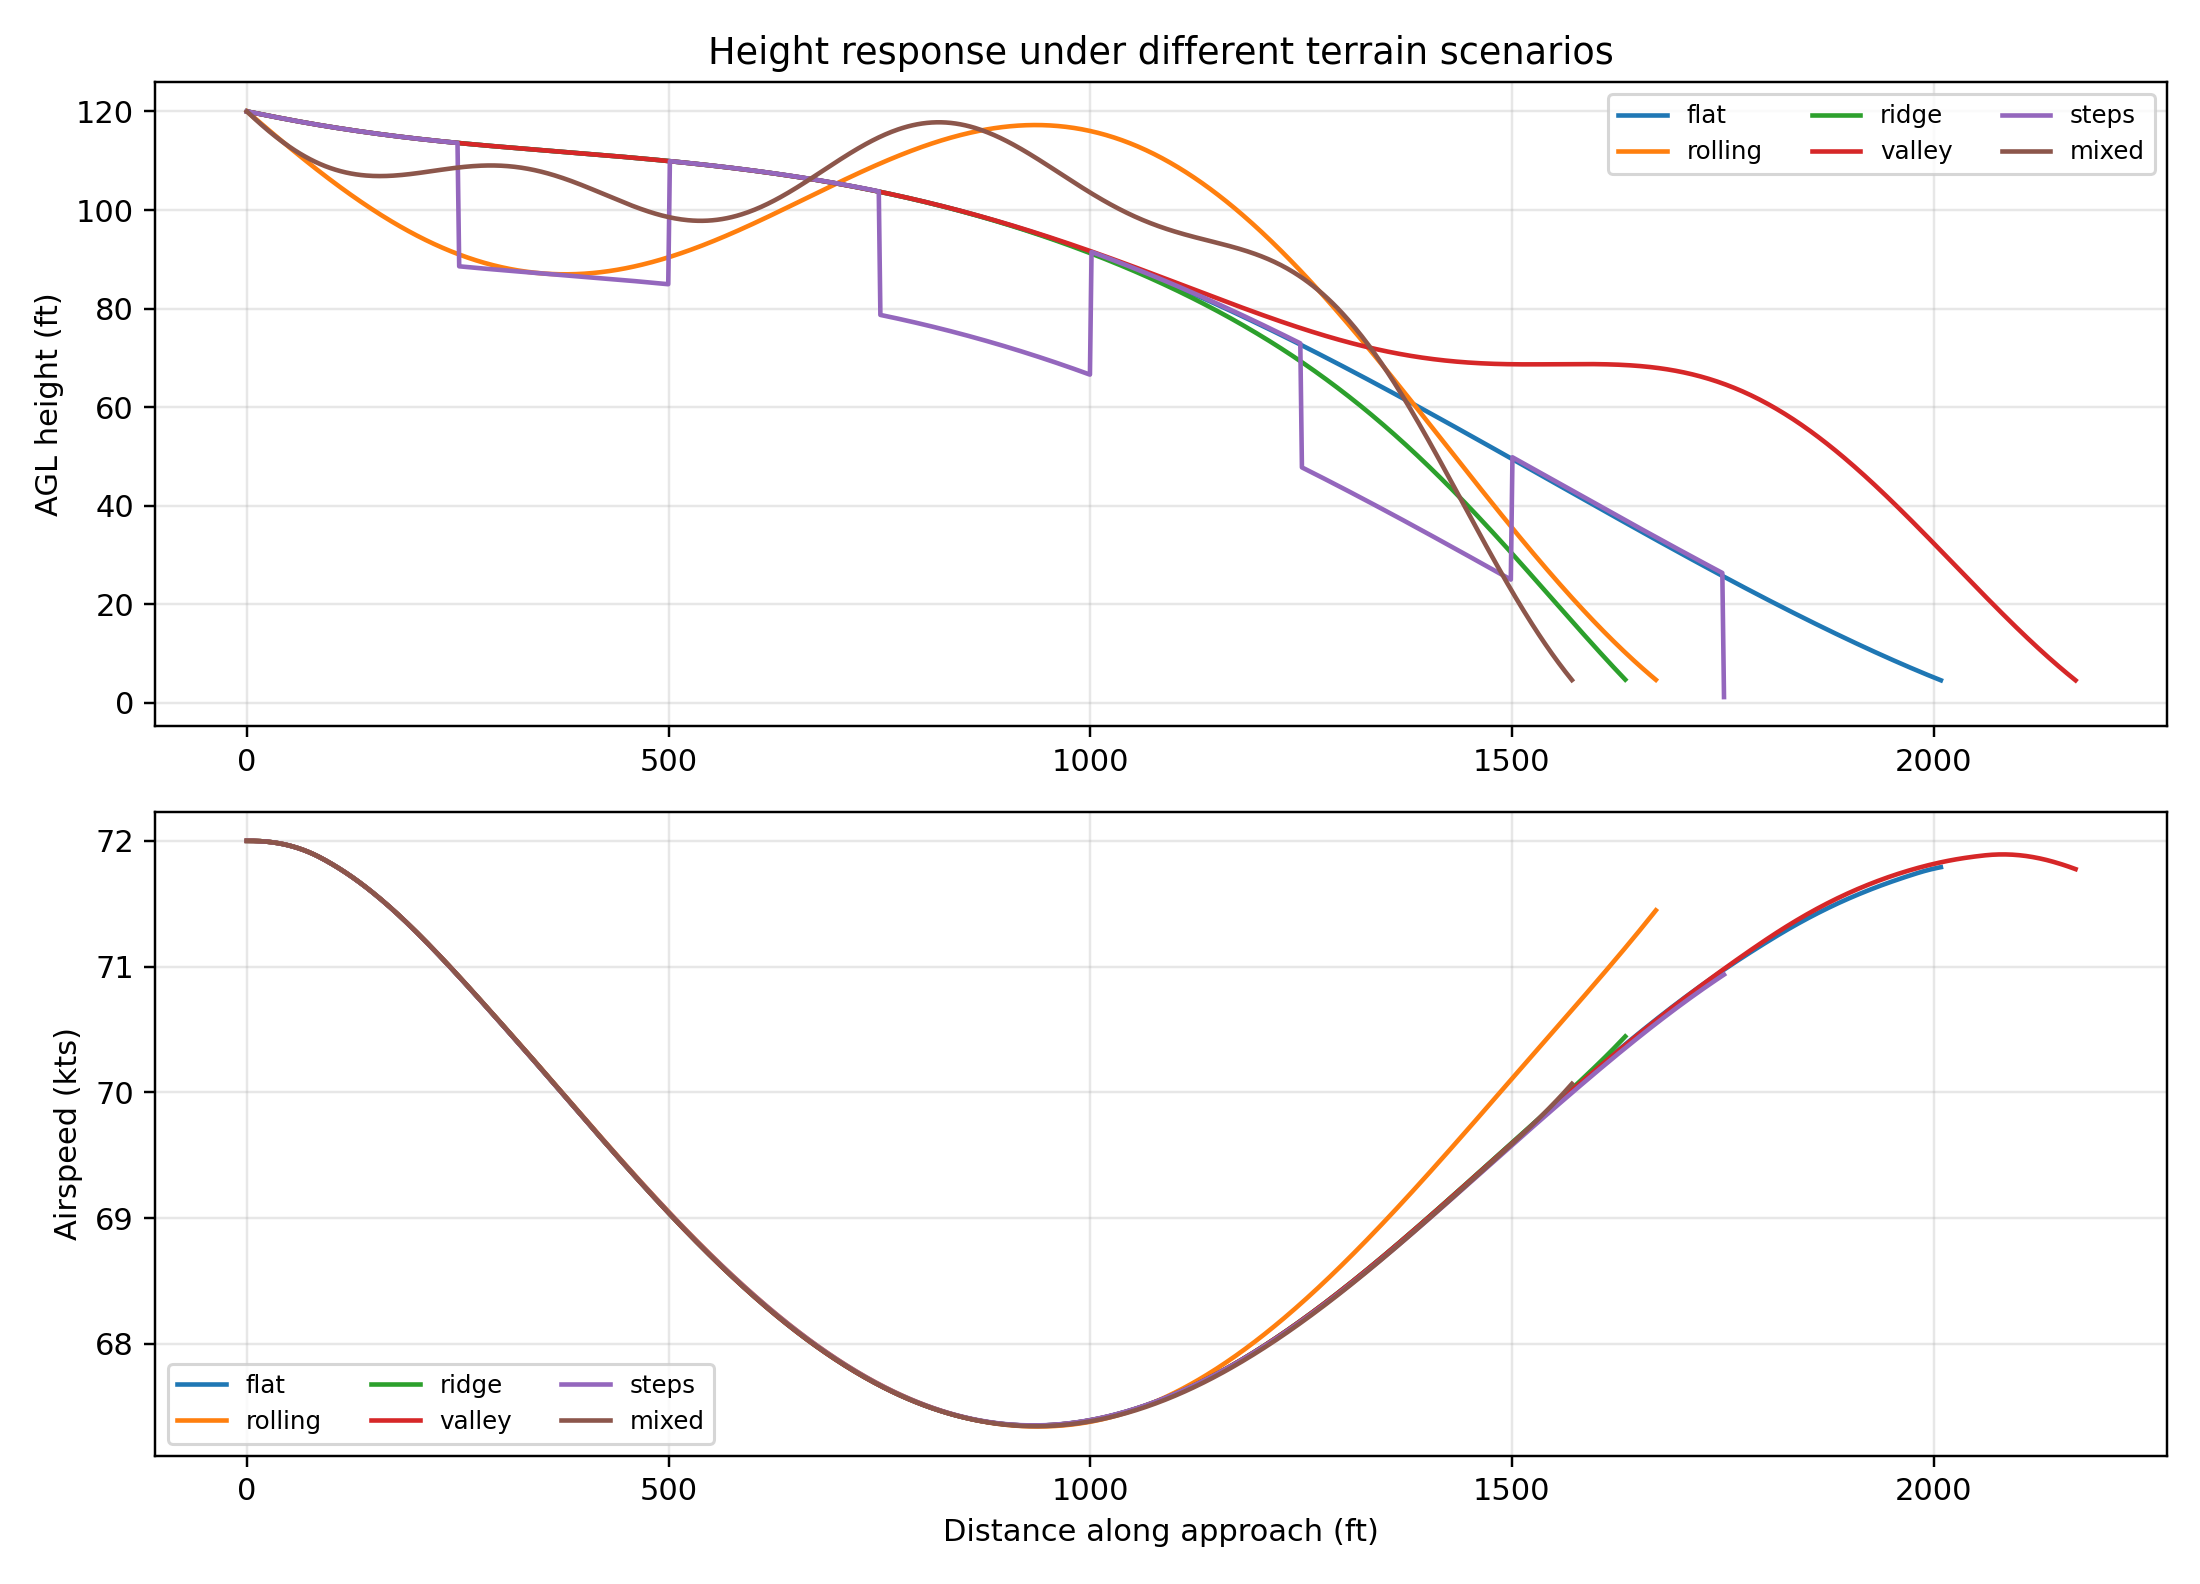
\includegraphics[width=5.45in,height=0.66\textheight,keepaspectratio]{images/image13.png}
\caption{不同地形工况下离地高度与空速响应对比}
\label{fig:5-1}
\end{figure}

就速度保持规律而言，在各个工况下飞行器末段的速度，整体上都被控制在了安全范围之内，这表明系统大体上能够达成速度约束这项任务。不过不同地形条件下速度调节的难度存在差异。在平坦地形、谷地地形工况里，速度变化相对比较平稳顺利，末段速度保持的效果比较理想，在起伏地形和山脊地形工况中，因为要同时兼顾高度修正、姿态调整，速度波动有一定程度的增加，在阶跃地形工况中，尽管速度没有显著超出界限，然而由于近地阶段高度变化更为突然，速度控制与姿态控制之间协调的压力明显更大。

依据姿态变化规律来分析，在平坦地形工况里，俯仰角、滚转角的变化幅度是最小的，这意味着系统于标准着陆条件下能够维持较好的纵横向稳定性。在起伏地形与山脊地形工况当中，飞行器为了持续对下滑状态、跑道对准进行修正，俯仰角跟滚转角的波动会更加明显。在谷地地形工况中，俯仰角整体来说比较平顺，然而滚转角呈现出一定的偏转特征，这表明其横向稳定性受到了地形的影响。在阶跃地形工况中，姿态修正最为频繁，这体现出系统需要在较短时间内同时兼顾高度、速度、方向的控制。可以看出，地形越是复杂，着陆末段状态变化就越敏感，系统对于操纵辅助、风险提示的需求也就越强。

\section{不利工况与较优工况识别}

按照之前所建立的评价指标与判据，能够对五类工况的优劣予以识别。从末段AGL、末段速度、俯仰角、滚转角、控制过程平顺性这几个方面进行综合考量，平坦地形工况的整体表现最为出色，能够当作较优工况。在该工况下，飞行器沿着预定的轨迹稳定下降，末段离地高度大概是4.60
ft，末段速度约为71.80
kts，俯仰角、滚转角都处于相对稳定的水平，这表明系统在标准环境中具备较好的收敛性与稳定性。

图~\ref{fig:5-2}从最大侧偏、最大下沉率和告警占比三个维度对比了不同地形工况下的系统表现，可作为安全性与稳定性的综合评价依据。

\begin{figure}[H]
\centering
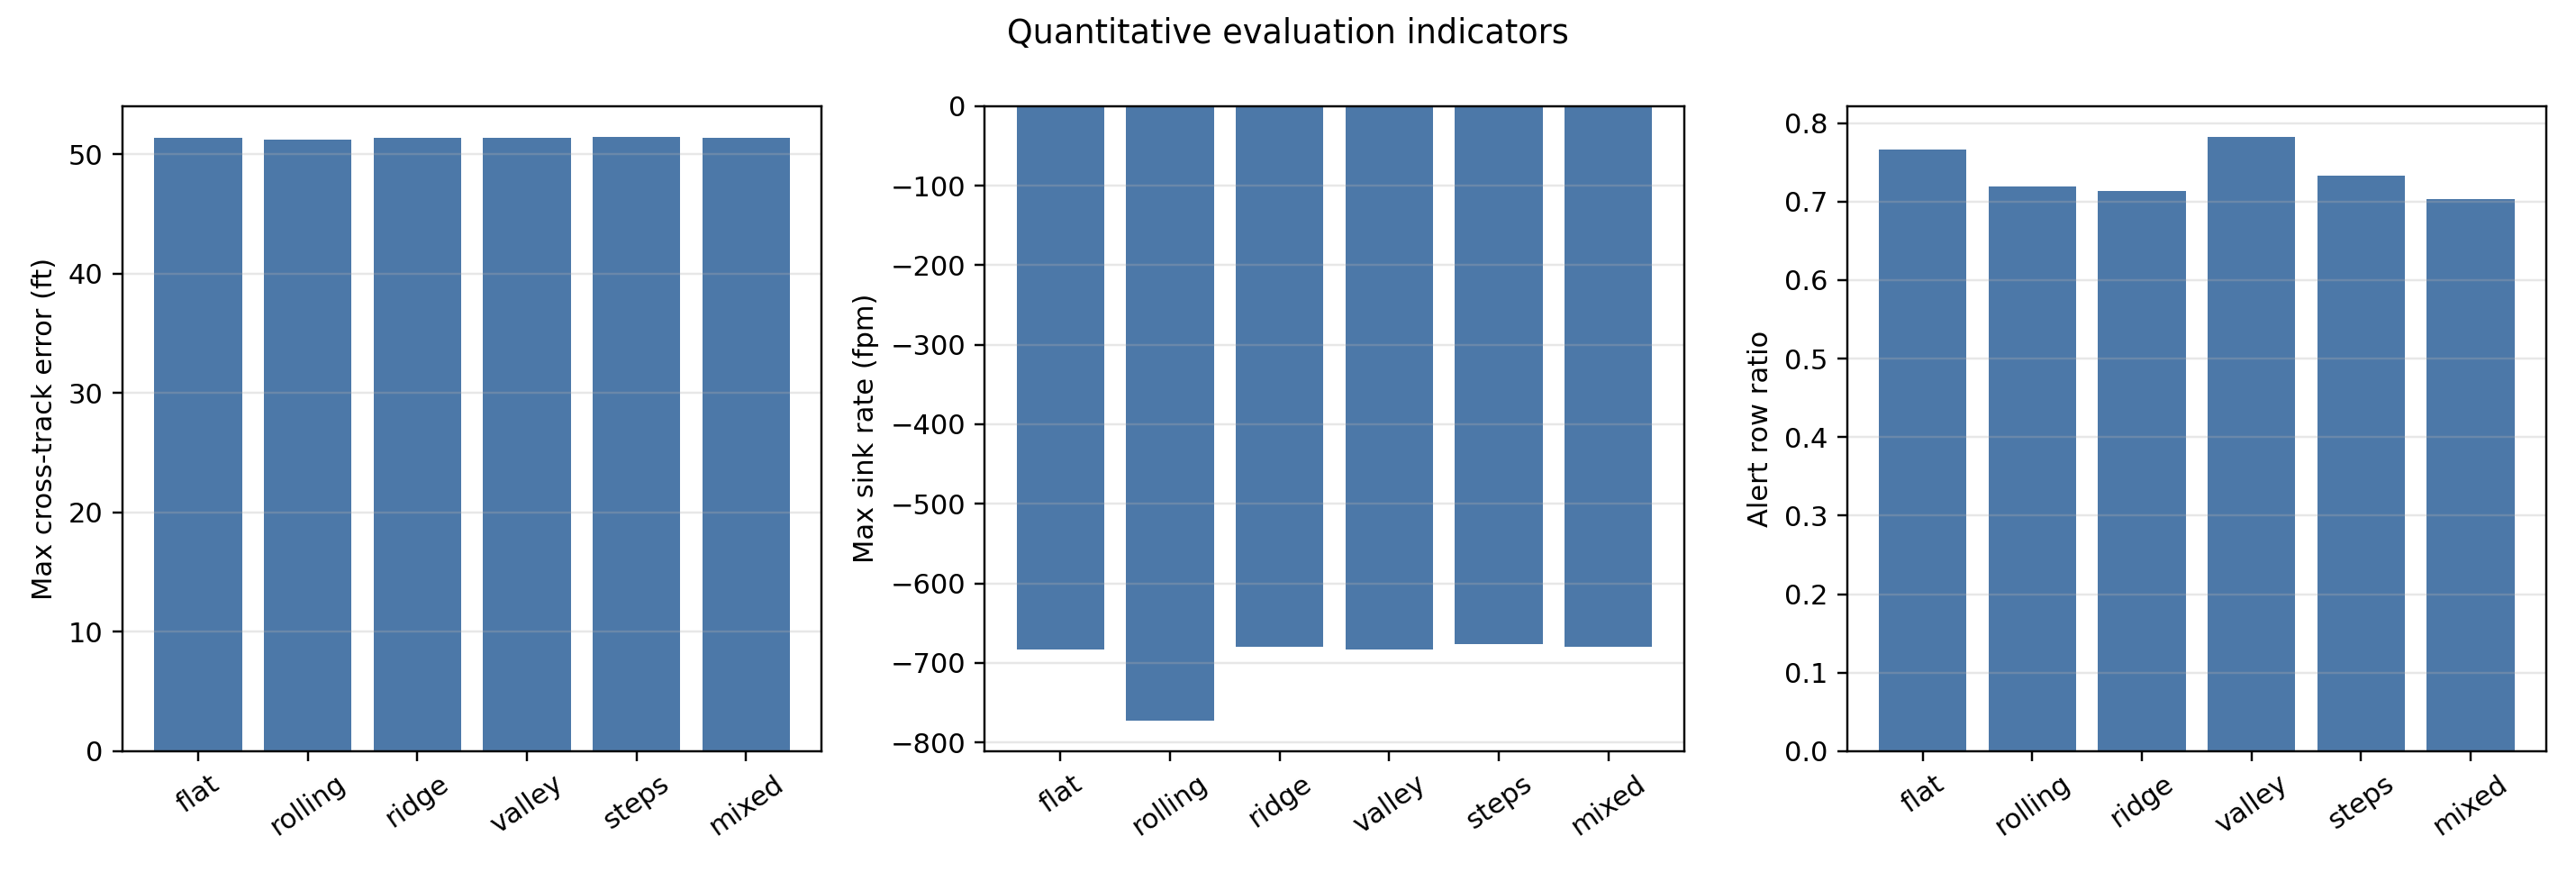
\includegraphics[width=0.92\linewidth,height=0.66\textheight,keepaspectratio]{images/image14.png}
\caption{多地形工况下关键评价指标对比}
\label{fig:5-2}
\end{figure}

谷地地形工况的仿真总时长比较长，不过末段速度保持的效果不错，末段离地高度和平坦地形相近，俯仰角的变化也比较小，故而总体性能比较理想，可当作次优工况。该工况的主要特点是前段控制裕度大，系统能较去进行轨迹修正，所以末段状态总体比较平顺。

起伏地形工况、山脊地形工况能够被归结为偏不利的工况类型。在起伏地形工况之中，俯仰角、滚转角所产生的变化幅度相对较大，这意味着系统需要持续地对处于连续变化状态的地面高程作出响应。而在山脊地形工况下，鉴于地形在接近区域呈现出快速抬升的趋势，飞行器相对离地高度的减小速度更为迅速，倘若控制修正稍微出现滞后的情况，便极易对拉平质量产生影响。所以，这两种工况尽管并未导致明显的失稳现象发生，却已然比较暴露出系统在复杂环境下所存在的薄弱环节。

在各种工况中，阶跃地形工况可被判定为最为不利的工况。其最为突出的一个特征在于，末段AGL仅仅约为1.20
ft，这一数值明显低于其他工况的相应数值，这说明地形发生突变后，近地阶段的控制调整空间被极大幅度地压缩了。该工况末段滚转角的绝对值相对比较大，这表明横向姿态保持的难度也随之增大了。虽说速度并没有出现严重越界的情况，但是高度突变对于操纵者判断拉平时机、接地窗口造成了比较明显的干扰。所以，在后续进行人机交互强化策略分析、系统优化的时候，阶跃地形工况是需要重点予以关注的对象。

\section{典型工况机理解释}

平坦地形工况能够呈现出比较优异的工况表现，其主要缘由在于地面高程基本维持恒定状态，飞行器海拔高度与相对离地高度之间的关系清晰明了且简单易懂，系统能够依据预先设定的下滑角、目标速度、阶段切换规则实现稳定运行，操纵者对于末段接地时机的判断也更易于与系统提示达成一致，如此一来整体控制便最容易趋向收敛。

为能更详细地说明控制器在典型工况下的行为表现，图~\ref{fig:5-3}展示出俯仰角、滚转角、升降舵、油门指令同步变化的情况，以此来呈现控制器完成下滑、修正、接地这一系列连贯动作的方式。比如，在下滑阶段，油门和升降舵共同作用去维持目标空速、下滑角，在拉平阶段，升降舵上偏的指令会使飞行器抬头，从而减小下沉率。

\begin{figure}[H]
\centering
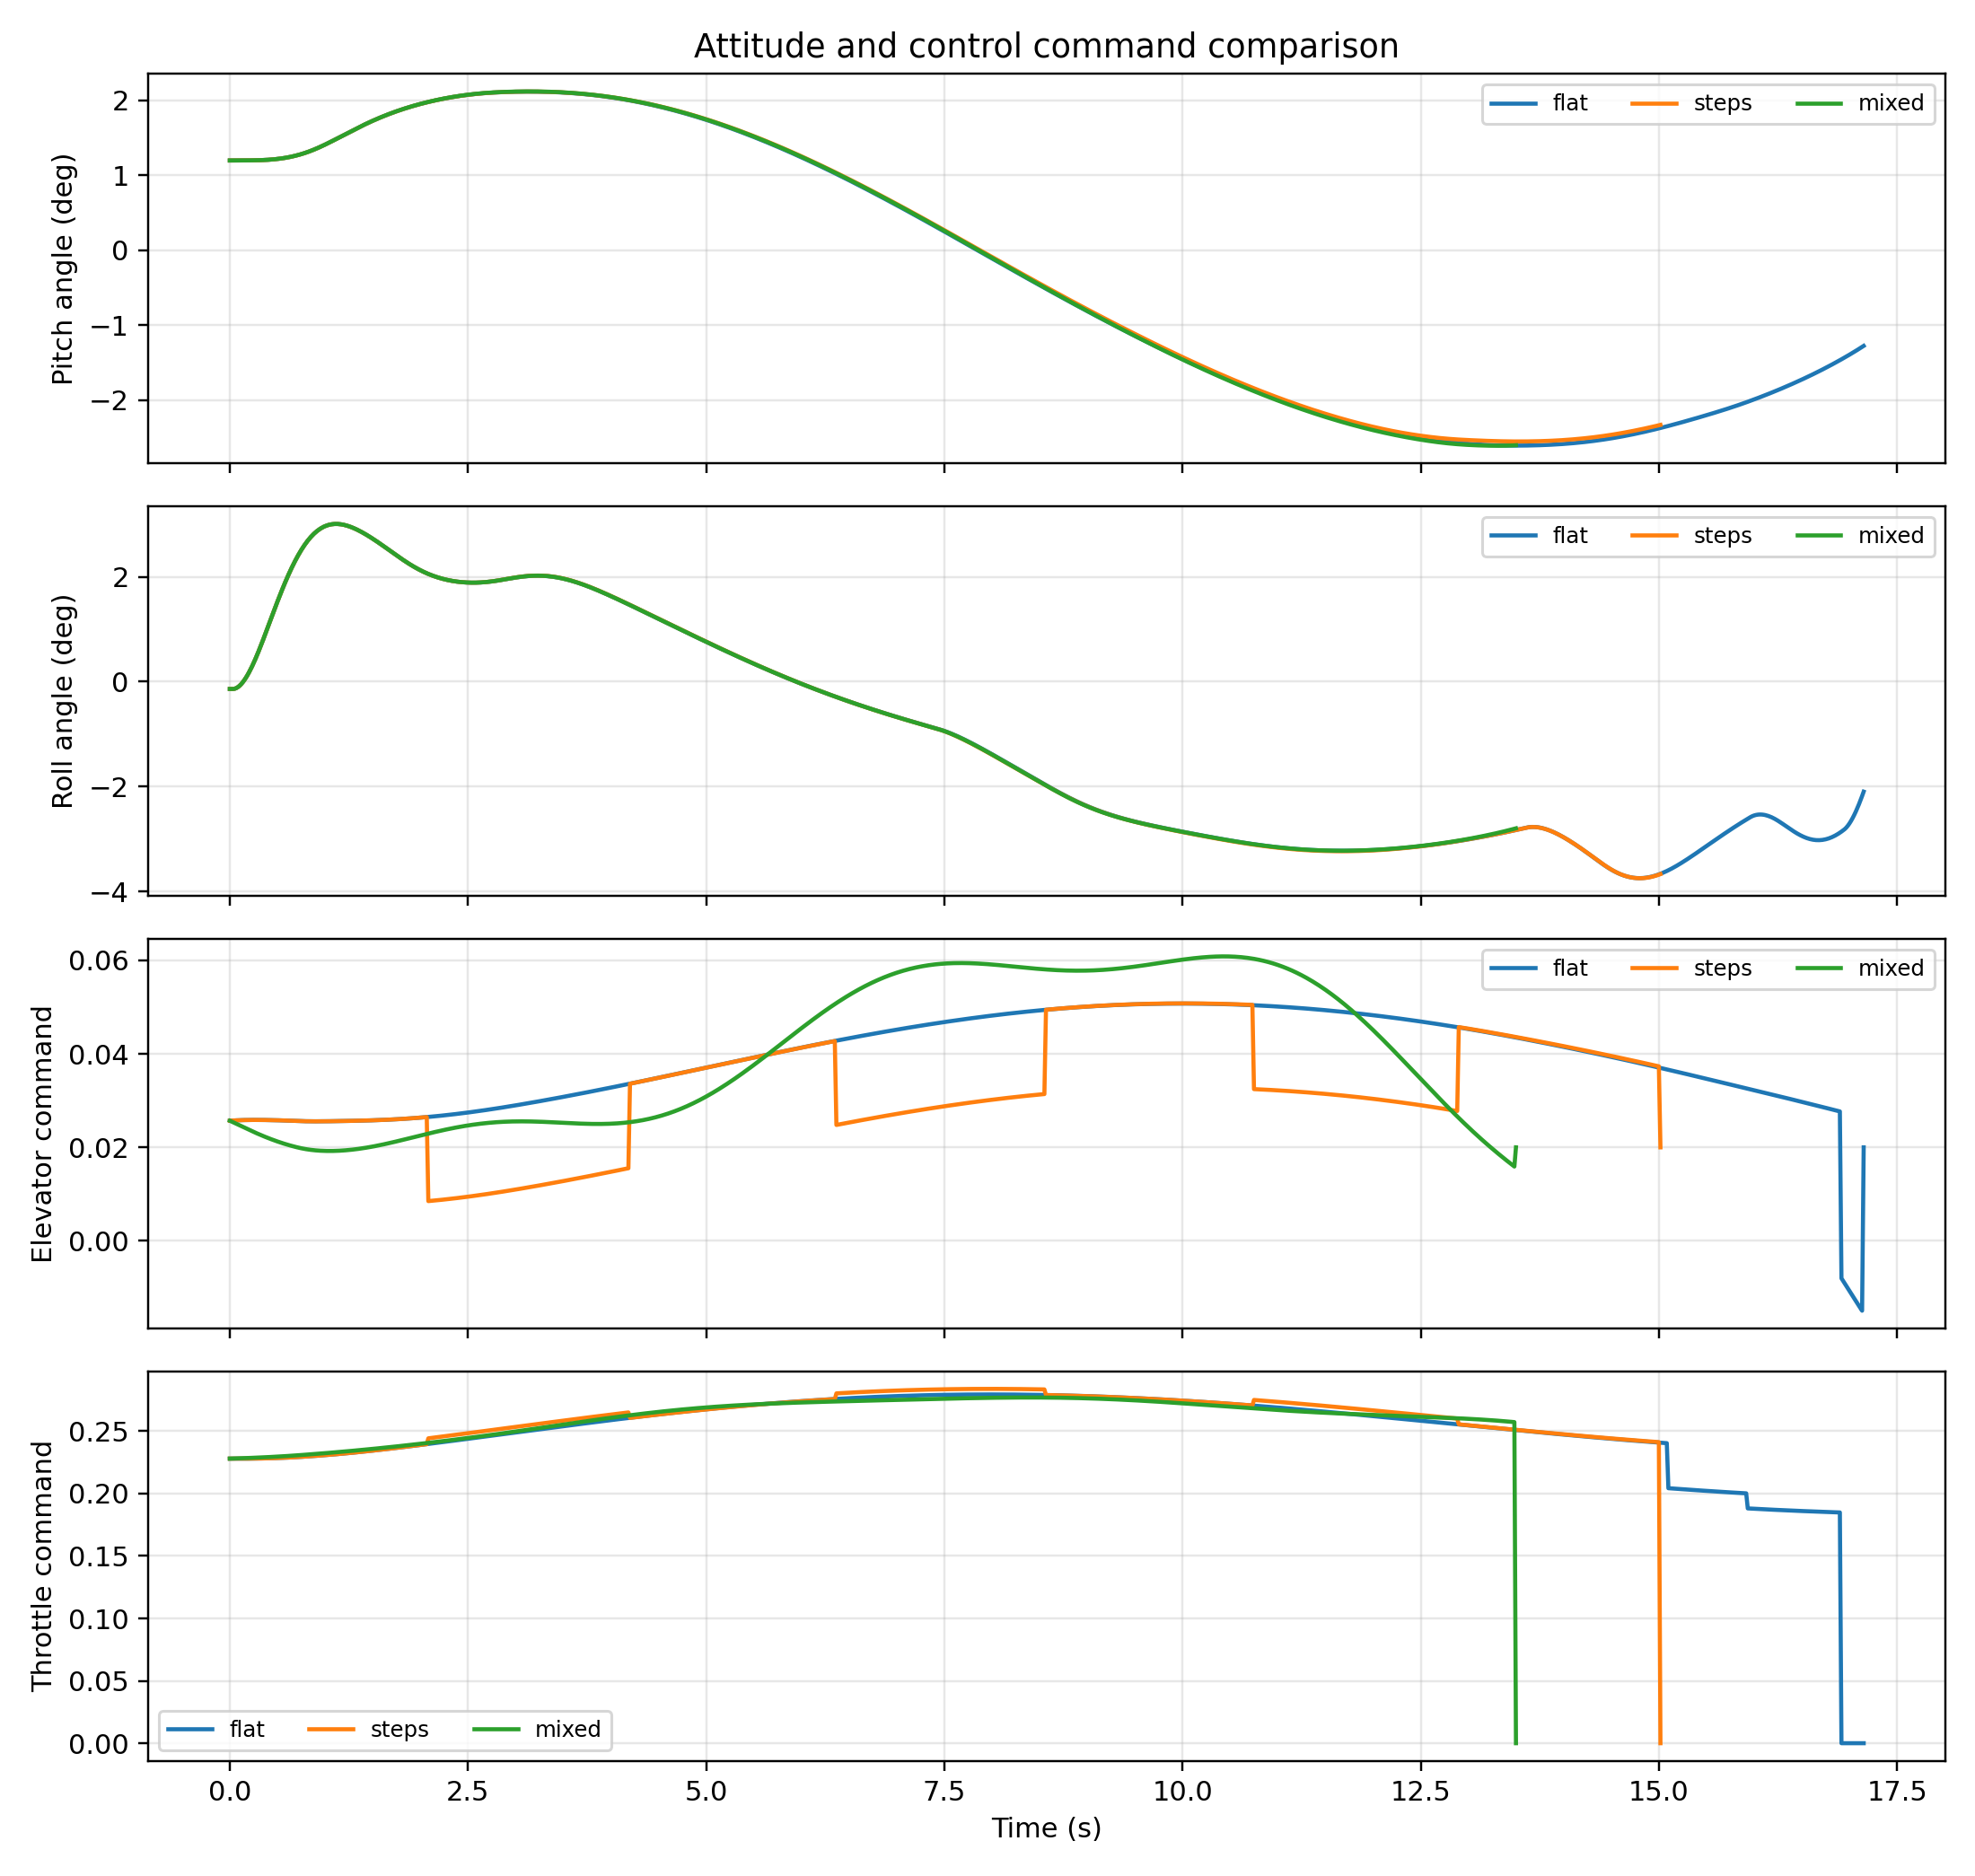
\includegraphics[width=3.99in,height=0.66\textheight,keepaspectratio]{images/image15.png}
\caption{典型工况下姿态角与控制指令变化}
\label{fig:5-3}
\end{figure}

山脊地形工况所存在的问题主要是因为在接近跑道之前地面高程迅速上升。飞行器海拔高度尽管依旧平稳下降，然而其相对离地高度会在较短时间内急剧减小，使得系统必须更早地完成下沉率抑制、姿态修正。要是修正速度偏慢，就容易导致拉平不足的情况发生，要是修正过度，又有可能致使姿态波动有所增加。山脊地形工况体现出系统对于地形的快速变化比较敏感。

阶跃地形工况被认为是最不利的，其根本缘由是地面高程的不连续变化使得飞行器相对离地高度突然降低。对于操纵者来说这种情况会压缩反应时间，而对于控制系统而言则会加大阶段识别、边界判断、接地时机控制的难度。也就是说这种工况并非只是纵向控制困难，而是高度判断、姿态控制、接地窗口识别同时变得困难。所以在复杂地形特别是阶跃型地形条件下，仅仅依靠基础控制律难以充分确保着陆品质，还需要借助更清晰的状态提示、风险告警、约束保护来提高系统鲁棒性。

综合来看，通过多工况分析能够发现，平坦地形能够当作系统的基准参考，谷地地形整体呈现出较好的状况，起伏、山脊、阶跃地形则更能够体现系统在复杂环境下的风险特性。其中，阶跃地形属于最为典型的不利工况，应当作为后续人机交互强化设计、系统优化时重点分析的对象。
